\chapter{Introducción}
Las redes de sensores inalámbricos (WSN, por sus siglas en inglés) habilitan la interacción con el mundo físico mediante pequeños nodos que de manera automática se organizan para reunir información sensorial, procesar datos y comunicarse inalámbricamente\cite{ yick:wsn_survey}. Se componen de nodos de \textit{bajo alcance}, de \textit{bajo costo}, y de \textit{bajo consumo de energía} que pueden ser desplegados en áreas domésticas, urbanas, hostiles, lejanas o de difícil acceso para reunir información de un ambiente o fenómeno determinado. Los nodos en una WSN son dispositivos con escasa memoria y baja capacidad de procesamiento que operan principalmente con baterías, equipados con uno o más sensores, una unidad de procesamiento, memoria y radio comunicación.

Dadas las características ofrecidas por las WSN el desarrollo de aplicaciones encuentra un gran potencial en áreas tales como \textit{seguridad}, \textit{rastreo}, \textit{medicina} y \textit{monitoreo ambiental}. En aplicaciones de seguridad, sensores desplegados en zonas bajo vigilancia pueden detectar intrusiones, monitorear niveles de radiación y detectar la presencia de líquidos o gases tóxicos\cite{sun:bordersense, simon:sniper}. Es posible rastrear, localizar y verificar las condiciones de paquetes en servicios de mensajería, rastrear vehículos y detectar la presencia de seres humanos. El desarrollo de redes inalámbricas corporales permite que sensores se encarguen de monitorear los signos vitales de pacientes en un hospital y generar alarmas cuando las variables médicas han superado valores críticos\cite{ko:healthcare, redondi:laura}. Así mismo, edificios o casas inteligentes pueden ofrecer asistencia, como cambios de iluminación y ventilación, a partir de variaciones detectadas en el ambiente\cite{ spasova:wsn_aal}. Por último, existe un creciente interés en introducir sensores inalámbricos en los procesos industriales y de producción agrícola, monitorear el comportamiento de plantas o animales y generar alertas para la mitigación de riesgos por desastres naturales\cite{Zhao:wsn_industrial, anastasi:vinedo, corke:environmental, hart:esn}. 

Con frecuencia en las aplicaciones de WSN es necesario distribuir nodos en zonas de difícil acceso donde no es posible realizar ningún tipo de mantenimiento. Debido a esto, se debe garantizar la longevidad de los nodos utilizando novedosas técnicas para el ahorro de energía. Igualmente se debe considerar que, ante una posible pérdida de nodos o errores en la comunicación, las WSN deben ofrecer una gran tolerancia a fallos y mecanismos de recuperación. Estas directivas de diseño de las WSN están determinadas por el propósito de la red, de los recursos disponibles y del ambiente donde esta trabaje. En general, el diseño de aplicaciones con WSN se constituyen con software y dispositivos electrónicos \textit{ad-hoc} considerando el costo, el tiempo de vida y la utilidad de los componentes de la red. 

%%La naturaleza de una WSN ayuda a proveer redundancia en áreas con una alta densidad de sensores donde el fenómeno o variable de interés puede estar en el rango de observación y comunicación de más de un nodo de manera simultánea. Esta redundancia puede ser aprovechada obteniendo lecturas de nodos cercanos o definiendo nuevas rutas en la comunicación inalámbrica. 

En la mayoría de los casos, las WSN forman parte de un sistema mayor. La información sensorial generada en la red suele concentrarse en una estación base constituida principalmente por un sistema de almacenamiento y aplicaciones para la presentación de la información hacia el usuario. Para esto, un nodo \textit{colector de datos} o \textit{data sink} se encarga de reunir los datos de los sensores de la WSN y retransmitir la información hacia el exterior de la red, de esta forma provee a la red la habilidad de vincularse con otros sistemas heterogéneos de comunicación. El nodo colector de datos puede realizar procesamiento y generalmente funciona como \textit{coordinador} de la WSN, lo que implica una mayor carga de trabajo y consumo de energía, por lo tanto la plataforma de hardware de un colector de datos debe ser de mayor complejidad a diferencia de los demás nodos en la red. 

%%En el presente trabajo se describe el diseño e implementación de un dispositivo ad-hoc (hardware y software) que opera como un colector de datos reuniendo y retransmitiendo la información de la WSN hacia el exterior.

\section{Planteamiento del problema}

%El deslizamiento de laderas es uno de los fenómenos geológicos que frecuentemente expone la seguridad de la población. En el estado de Veracruz $2,318$ localidades se encuentran en riesgo clasificado como \textit{Muy Alto} y \textit{Alto}\cite{pc:siaver}. Aunque existen manifestaciones que indican una potencial ocurrencia de estos fenómenos, es complicado establecer con exactitud el momento cuando puede suceder un evento. Para ello, el monitoreo y la detección temprana pueden ser mecanismos que ayuden a reducir el riesgo\cite{cenapred:guia}. 

El Consejo Nacional de Ciencia y Tecnología (CONACyT) y el Consejo Veracruzano de Ciencia y Tecnología (COVECyT) han encargado al Laboratorio Nacional de Informática Avanzada LANIA A.C. el proyecto \textit{"Monitoreo remoto y detección en tiempo--real de deslaves y desgajamientos de tierra a causa de precipitaciones pluviales utilizando redes de sensores inalámbricos"} (FOMIX--VER--2010--C04--152366) que busca desarrollar una herramienta que permita observar el comportamiento de estos fenómenos y generar mensajes de alerta ante posibles incidentes. 

\begin{figure}
	\centering
	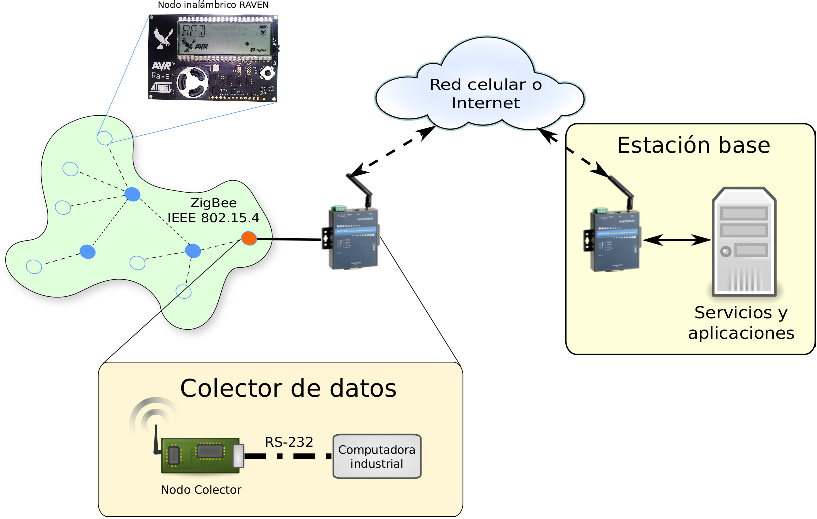
\includegraphics[scale=0.9]{capitulo_1_imgs/esquema_general.pdf} 
	\caption{Esquema general del proyecto}
	\label{fig:esquema_general}
\end{figure}

La figura \ref{fig:esquema_general} muestra una propuesta del esquema general del proyecto que considera tres componentes principales: 1) Una WSN que cumple con el estándar ZigBee IEEE 802.15.4\cite{zigbee:estandar}, 2) Un enlace de comunicación entre la WSN y una estación base remota a través del servicio de comunicación GPRS (\textit{General Packet Radio Service}) y 3) un conjunto de servicios y aplicaciones de almacenamiento y presentación de información hacia el usuario. Mediante sensores instalados en puntos críticos como laderas cercanas a zonas urbanas, carreteras o líneas de energía, se plantea recoletar información de humedad del suelo, inclinación, distancia y precipitación pluvial. 

Se requiere que la WSN pueda ser instalada tanto en zonas urbanas como rurales, con acceso remoto desde cualquier parte mediante Internet; debido a la cobertura que ofrece, se sugiere utilizar al servicio GPRS como medio de transporte. En particular, se propone utilizar una computadora embebida industrial con interfaces de comunicación Ethernet, RS-232 y GPRS para el acceso a Internet, sin embargo, se carece de un enlace de comunicación entre la WSN y esta computadora.

%Se requiere que la WSN pueda ser instalada tanto en zonas urbanas como rurales, con acceso remoto desde cualquier parte mediante Internet; debido a la cobertura que ofrece, se sugiere utilizar a la red celular GPRS (\textit{General Packet Radio Service}) como medio de transporte. En particular se propone utilizar una computadora embebida industrial con interfaces de comunicación Ethernet, RS-232 y GPRS, en conjunto con un circuito electrónico ad-hoc que funcione como puente de comunicación entre la WSN y esta computadora industrial. 
Por lo tanto en este trabajo se plantea diseñar e implementar un dispositivo ad-hoc que comunique una WSN usando los estándares IEEE 802.15.4 y ZigBee con una computadora industrial a través de la interfaz RS-232 y de esta forma, implementar un colector  de datos para esta aplicación. 

%Particularmente se plantea diseñar e implementar un dispositivo que comunique a una WSN usando el estándar ZigBee IEEE 802.15.4 con una computadora embebida industrial a través de la interfaz RS-232, y de esta forma, implementar un colector de datos para esta aplicación. 

\section{Objetivo}

Diseñar e implementar un sistema (hardware y software) que permita realizar la comunicación entre una WSN que cumple con el estándar ZigBee IEEE 802.15.4 y una computadora embebida industrial a través de la interfaz RS-232. 

\subsection{Objetivos espec\'ificos}

\begin{enumerate}
	\item Diseñar e implementar el circuito electrónico conversor de comunicación Serial RS-232 a ZigBee IEEE 802.15.4,
	\item Definir un protocolo de comunicación para la transferencia bidireccional de información entre el dispositivo y la computadora embebida industrial,
	\item Implementar el software de comunicación embebido para el dispositivo, 
	\item Implementar un conjunto de instrucciones para utilizar el dispositivo desde la computadora embebida industrial, 
	\item Desarrollar una aplicación para demostrar del funcionamiento de todos los componentes. 
\end{enumerate}

\section{Justificaci\'on} 

La utilidad de una WSN se puede ver gravemente limitada si los usuarios no cuentan con los mecanismos para tener acceso a la red con la finalidad de extraer datos de los sensores, configurar parámetros de funcionamiento, activar nodos individualmente, verificar el estado de funcionamiento de cada nodo y verificar el funcionamiento del sistema de comunicación de la WSN.

Puesto que una WSN opera con un protocolo particular de comunicación es necesario proveer interfaces de hardware y software que permitan de manera transparente facilitar la comunicación entre tecnologías que utilizan distintos protocolos de comunicación.  

\section{Estructura del documento}

El desarrollo de este trabajo tiene la siguiente estructura: 

\begin{itemize}
	\item \textbf{Capítulo 2 :} Se introducen conceptos sobre las WSN y sus principales componentes. Se mencionan las distintas tecnologías que se utilizarán en el desarrollo de este trabajo,
	\item \textbf{Capítulo 3 :} Se describe el diseño del dispositivo, se mencionan los requerimientos de la aplicación y se muestra el diseño del circuito y del software embebido,
	\item \textbf{Capítulo 4 :} Se describen los escenarios de pruebas para el dispositivo y se muestran los resultados obtenidos. 
	\item \textbf{Capítulo 5 :} Se mencionan las conclusiones obtenidas a partir de los resultados observados y trabajo a futuro. 
\end{itemize}